% This is samplepaper.tex, a sample chapter demonstrating the
% LLNCS macro package for Springer Computer Science proceedings;
% Version 2.21 of 2022/01/12
%
\documentclass[runningheads]{llncs}
%
\usepackage{comment}
\usepackage{xcolor}%
\usepackage{textcomp}%
\usepackage{manyfoot}%
\usepackage{booktabs}%
\usepackage{algorithm}%
\usepackage{algorithmicx}%
\usepackage{algpseudocode}%
\usepackage{listings}%
\usepackage{tikz}
\usepackage{color}
\usetikzlibrary{chains,matrix,scopes,shapes.geometric}
\usepackage{hyperref}
\usepackage{footnote}
\usepackage{todonotes}
\usepackage[utf8]{inputenc}

\usepackage[T1]{fontenc}
% T1 fonts will be used to generate the final print and online PDFs,
% so please use T1 fonts in your manuscript whenever possible.
% Other font encondings may result in incorrect chara cters.
%
\usepackage{graphicx}
\sloppy
% Used for displaying a sample figure. If possible, figure files should
% be included in EPS format.
%
% If you use the hyperref package, please uncomment the following two lines
% to display URLs in blue roman font according to Springer's eBook style:
%\usepackage{color}
%\renewcommand\UrlFont{\color{blue}\rmfamily}
%\urlstyle{rm}
%
\begin{document}
%
\title{Automated Creation of the Legal Knowledge Graph Addressing Legislation on Violence Against Women: Resource, Methodology and Lessons Learned}
%\title{Automated Legal Knowledge Graph Generation  Addressing Legislation on Violence Against Women}
%
\titlerunning{Automated Creation of the Legal Knowledge Graph}
% If the paper title is too long for the running head, you can set
% an abbreviated paper title here
%
\author{Claudia d'Amato\inst{1}\orcidID{0000-0002-3385-987X} \and
Giuseppe Rubini\inst{1} \and
Didio Franceso\inst{1}\and
Francioso Donato\inst{1}\and
Fatima Zahra Amara\inst{1}\orcidID{0000-0001-8463-0330}\and
Nicola Fanizzi\inst{1}\orcidID{0000-0001-5319-7933}}
%
\authorrunning{C. d'Amato et al.}
% First names are abbreviated in the running head.
% If there are more than two authors, 'et al.' is used.
%
\institute{Computer Science Department, University of Bari Aldo Moro, Italy
\email{\{claudia.damato, fatima.amara, nicola.fanizzi\}@uniba.it}\\
\email{\{g.rubini13, f.didio2, d.francioso7\}@studenti.uniba.it}}
%
\maketitle 
\begin{abstract}
Legal decision-making process requires the availability of comprehensive and detailed legislative background knowledge and %as well as 
up-to-date information on legal cases and related sentences/decisions. Legal Knowledge Graphs (KGs) would be a valuable tool to facilitate access to legal information, to be queried and exploited for the purpose, and to enable advanced reasoning and machine learning applications. %besides being made available as 
Indeed, legal KGs may act as %as well as an important 
knowledge intensive component to be %also 
used by predictive machine learning solutions supporting the decision process of the legal expert. Nevertheless, a few KGs can be found in the legal domain. To fill this gap, %in this paper we introduce 
we developed a legal KG targeting legal cases of violence against women, along with clear adopted methodologies. 
%Our primary goal is the development of structured and enriched legal KGs that facilitate access to legal information and enable advanced reasoning and machine learning applications. 
Specifically, the paper introduces two complementary %methodologies 
approaches for automated legal KG construction; a systematic bottom-up approach, customized for the legal domain, and a new solution leveraging Large Language Models. Starting from legal sentences publicly available from the European Court of Justice, % that are publicly available, 
the solutions integrate structured data extraction, ontology development, and semantic enrichment to produce KGs tailored for legal cases involving violence against women. After analyzing and comparing the results of the two approaches, the developed KGs are validated via suitable competency questions. 
The obtained KG may be impactful for multiple purposes: can improve the accessibility to legal information both to humans and machine, can enable complex queries and may constitute an important knowledge component to be possibly exploited by machine learning tools tailored for predictive justice.\\ 
\textbf{Resource type:} Knowledge Graphs\\
\textbf{License:} Creative Commons Attribution 4.0 International \\
\textbf{DOI:} \url{https://doi.org/10.5281/zenodo.15270173} \\
\textbf{URL:} \url{https://lod-cloud.net/dataset/PREJUST4WOMAN\_PROJECT}
\keywords{Knowledge Engineering \and Large Language Models \and Knowledge Graph Generation \and Linked Data \and Semantic Web \and Violence Against Women \and Predictive Justice.}
\end{abstract}

\section{Introduction}
In recent years, the legal domain has been interested by an increasing usage of Artificial Intelligence (AI) solutions \cite{diPorto2024,li2024construction} to effectively manage and mine legal consultation and decision process. %However, 
Despite %significant 
advancement in legal technologies~\cite{Westermann19}, a significant gap exists in the availability of structured and easy to query resources tailored to the legal domain such as Knowledge Graphs (KGs)~\cite{hogan2022knowledge}. Existing KGs in the legal domain often fail to address nuanced and domain-specific challenges, including the need for interoperability, semantic richness, and adaptability to predictive justice applications \cite{changyue_wang__2024,xuran_wang__2024}.
%\todo{@FATIMA: this assertion needs to be substantiated with appropriate references supporting it} 
%Indeed, 
A legal KG needs to be able to cope with the specific and intricate writing style of laws and sentences, and %as well as needs to able to 
keeping  track of the evolution of laws, including exceptions and applicability.

We specifically focus on the widespread and urgent issue of violence against women\footnote{\url{https://www.who.int/news-room/fact-sheets/detail/violence-against-women}}  %is a widespread and urgent issue 
that leads to physical and mental health problems, economic losses and social instability~\cite{dawa2022violence} and that impacts societies around the world. Manifesting in physical and emotional forms, it constitutes a grave violation of human rights, threatening the safety, dignity, and well-being of countless women. 
%
%While addressing violence against women is critical, some argue that existing initiatives may be insufficient or poorly implemented, highlighting the need for ongoing evaluation and adaptation of policies to ensure that they effectively meet the needs of victims and prevent future violence \cite{tuba_trkkan__2023}.
%Targeting this issue requires dismantling patriarchal structures and implementing prevention strategies such as empowerment programs, education, community mobilization, and accessible support services. 
Actually, a multifaceted approach involving governments, civil society and individuals is essential to counter this pervasive problem and promote healthier and more equitable societies. 
Our work aims to contribute to this effort by developing advanced instruments and knowledge components to assist in the legal handling of cases related to violence against women. %and to possibly support more effective prevention and intervention strategies. 
%
%Manifesting in physical and emotional forms, it constitutes a grave violation of human rights, threatening the safety, dignity, and well-being of countless women. %Rooted in persistent gender inequalities, this pervasive problem remains a critical challenge for legal systems and human rights defenders alike. 
%
%Specifically, addressing 
This %present issue 
goal requires robust %legal 
tools %and frameworks 
capable of supporting legislative interpretation, judicial decision-making, policy formulation %. %Despite advancement in legal technologies~\cite{Westermann19}, a significant gap exists in the availability of structured resources tailored to cases of gender-based violence, particularly in the domain of KG engineering. 
%as well as 
and access to structured resources, in the form of KGs, tailored to cases of gender-based violence. 
%
%Existing KGs in the legal domain often fail to address nuanced and domain-specific challenges, including the need for interoperability, semantic richness, and adaptability to predictive justice applications\cite{xuran_wang__2024} \cite{changyue_wang__2024}.
%\todo{@FATIMA: this assertion needs to be substantiated with appropriate references supporting it} 
%Indeed, a legal KG needs to be able to cope with the specific and intricate writing style of laws and sentences, as well as needs to able to keep  track of the evolution of laws, including exceptions and applicability. 
%
%To address these gaps, %challenges, 
%
For this purpose, %with this paper 
we introduce a novel %resource, namely 
Legal KG, specifically designed to address legislation and judicial cases related to violence against women, jointly with methodologies adopted for its development. %, %. This work is part of the PREJUST4WOMEN project, which leverages advanced technologies, particularly in the fields of KG~\cite{hogan2022knowledge} generation and Artificial Intelligence (AI), to develop solutions 
%that aid in the legal handling of cases related to violence against women. 
%KGs are structured using triplets that have natural advantages in successfully organizing and logically structuring knowledge from various heterogeneous  sources \cite{peifeng2024joint}. The adoption of AI technology in the judicial domain has been extensively debated in academics \cite{li2024construction}. 


%The application of AI technology in the legal domain has been extensively discussed in the academic community \cite{li2024construction}.\\

The %main contribution presented in this work is the creation of 
Legal KG is automatically derived from the jurisprudence of sentences of the European Court of Human Rights (ECHR\footnote{\url{ https://www.echr.coe.int/}}), %, specifically 
targeting cases of gender-based violence, and it %is %. KGs are 
%designed to adhere 
adheres to the FAIR (\textit{Findable}, \textit{Accessible}, \textit{Interoperable}, \textit{Reusable}) data principles. %, ensuring that they are interoperable and structured for broad integration into existing legal and AI systems.
%
%Specifically, 
The resource is built upon two %complementary 
methodologies: a customization to the legal domain of the general KG development process%as proposed in
~\cite{Tamaauskaite2022} (that is a bottom-up solution %approach, a systematic method that combines 
combining data extraction, ontology development, and semantic enrichment via %. This approach ensures precision and 
alignment to domain-specific ontologies), %legal standards; 
and a new approach for automated KG generation, grounded on the exploitation of Large Language Models (LLMs) as the recent advancements have opened up new possibilities for automating and improving various phases of ontology development \cite{li2025large}, and %again 
customized to the legal domain. %LLM-based approach, customized to the legal domain, %; an innovative method leveraging the capabilities of state of the art AI models to automate KG generation. 
The two methodologies resulted complementary: the former providing more precise outcomes but more time-consuming, the latter more scalable but limited in accuracy.
The obtained resource has been also validated via suitable competency questions~\cite{Monfardini2023}. %, showing the validity. % of the resource itself.

%To the best of our knowledge, this work is the first dedicated initiative to develop a KG specifically addressing violence against women, thereby filling a critical gap in legal informatics. Beyond its direct contributions to this pressing issue, 
Besides the Legal KG being the first result addressing legislation,  particularly concerning violence against women, this resource may %also 
act as proxy %offers the resource offers valuable insights 
for broader applications. In the context of predictive justice, sentence prediction may be regarded as a link prediction problem on (a subset of) the Legal KG. This approach may be generalized to other domains in addition to the one of violence against women, provided the availability of legal KGs %intensive structured knowledge components 
generated  %and resources development in the legal domain targeting alternative issue, 
by adopting the proposed methodologies. %and societal challenges, establishing a foundation for future innovations in the field. 

The remainder of this paper is structured as follows: %Section~\ref{back} provides the necessary background for the proposed solution; % detailed overview on the background of the importance of addressing the issue of violence against women and the KG engineering advancements. 
Section~\ref{related} review the %current 
state of the art %and related research 
on legal informatics, KGs and ontologies in law. %and on construction of KGs more broadly. %and summarizes recent results on KG development processes  %creation of KGs, with a particular focus on the relevant domain. 
%Section~\ref{back} provides the necessary background.  %while % that is functional for the proposed solution;
Section~\ref{approach-bottomUp} presents a customization to the legal domain of the bottom-up KG development process %, %proposed methodologies and the 
%implementation details 
and the obtained %for building the
Legal KG. %, %, including the processes used to develop the resources. 
%while 
Section~\ref{approach-LLM} presents a new approach for automated KG generation, grounded on the exploitation of Large Language Models (LLMs) and %again 
customized to the legal domain, %implementation details and 
the obtained Legal KG.
Section~\ref{disc} discusses the results and %evaluating 
the effectiveness of the adopted methodologies. Section~\ref{conc} conclude the paper %by summarizing the contributions and 
%also suggesting 
and delineate future research directions. % for future research and development.


\section{Related Work}\label{related}
In this section, we survey the state of the art %examine recent key papers focused 
at the intersection of legal informatics, %and 
usage of KGs for the legal domain and development of ontologies and legal thesaurus initiatives. %, ontologies, and KGs. 
These studies explore methods for structuring legal data, applying automated reasoning, and extracting insights from legal texts. %We also briefly present %will incorporate recent 
%advancements in LLMs %large language models (LLMs) 
%for KG generation, aiming to improve the automation and semantic richness of legal knowledge representation.

%\textit{Li et al. (2024)} \cite{li2024construction} focuses on 
Legal knowledge extraction and presentation of %presents %offers 
the Joint Knowledge Enhancement Model (JKEM), which refines LLMs using a %revolutionary 
prefix-based strategy to improve knowledge extraction accuracy is proposed in~\cite{li2024construction}. %, attaining 90.92\% precision. 
Using this paradigm, the authors created the Chinese Legal Knowledge Graph (CLKG), which has 3480 knowledge triples but does not exploit any existing domain ontology. %and provides a systematic and complete resource for legal knowledge inference.
Similarly, %\textit{Zhao et al. (2024)}~\cite{zhao2024method} propose 
in~\cite{zhao2024method} a judicial case KG centered mostly on event elements, employing a joint event extraction model to mine entity and event information from digital case records is presented. Using the Dgraph graph database for storage and GraphQL for querying, this approach facilitates %intelligent 
retrieval, case analysis, and knowledge discovery but does not push on interlinking the resource with other existing resources. %, paving the way for large-scale implementation of intelligent justice systems and legal services.
Analogously, %\textit{Stavropoulou et al. (2020)} 
in ~\cite{stavropoulou2020architecting} %presents 
the ManyLaws platform is presented, %namely 
a Big Open Legal Data (BOLD) platform that provides advanced and customizable access to legal information across the EU. The platform offers services such as legal corpus research, law comparison, legislative alignment analysis, and legislative timelines visualization. By leveraging data analytics, text mining, %semantic analysis, 
and interactive visualization, the platform enhances accessibility and understanding of legal data for a wide range of users but it does not focus on data interlinking and semantic querying. %\textit{Wei et al. (2024)}~\cite{wei2024intelligent} presents an %intelligent 
An approach for automatic legal document generation based on KGs is presented in~\cite{wei2024intelligent}. The method improves generation efficiency, quality, and content integrity %-- achieving up to 92\% accuracy -- 
compared to traditional rule-based approaches, contributing to %. This contributes to 
increased automation and precision in legal document production but, it does not allow %focus on 
semantic query of legal documents. 

Focusing more on operational level, %\textit{Francesconi et al. (2023)}~\cite{francesconi2023patterns} 
Francesconi et al.~\cite{francesconi2023patterns} presented a %novel approach 
solution for legal compliance checking % within the Semantic Web, utilizing ontology
by exploiting ontologies.  Specifically, classes and property restrictions are used to model deontic norms. %This solution %approach 
%addresses the challenge of norm defeasibility and employs decidable fragments of OWL2 for implementation. 
Legal reasoning is performed by decidable reasoners, and the framework is generalized through reusable patterns for modeling deontic norms and compliance verification. %\textit{Oliveira et al. (2024)}~\cite{oliveira2024rdf} propose 
An RDF-based graph for representing and searching specific parts of legal documents, such as paragraphs and clauses, rather than retrieving entire documents is formulated in~\cite{oliveira2024rdf}. The graph, grounded in an ontological framework, models both the general structure of the legal system and the internal composition of legal documents. This enables the efficient retrieval of relevant legal frameworks for specific topics. Nevertheless, the resource comes from a significant manual effort with limited automation of its construction. 

As for %the development of 
KGs in the legal domain, a seminal example has been developed within %is represented by %\textit{Schneider et al. (2022) }~\cite{schneider2022lynx} discuss 
the Lynx project~\cite{schneider2022lynx}, that focusing on GDPR regulation and contract compliance, %which aims to address the underdeveloped area of KG design in the legal domain. They introduce a Legal 
developed a KG\footnote{\url{https://lynx-project.eu/doc/lkg/}} %(LKG) 
that structures document relationships and incorporates legal linguistic information. %, thus filling a critical gap in legal resources.
Inspired by the Lynx project, %\textit{Anelli et al.}~\cite{Anelli23} proposed %\textbf{Official Italian State Mint} In the system presented in~\cite{Anelli23} 
a pipeline %was devised 
for extracting information from documents produced by the \textit{Istituto Poligrafico Zecca dello Stato} in order to make them easy to query is formulated in~\cite{Anelli23}. The system consists of multiple  %following 
modules, %: Law description extractor, Law description converter, Triple store, Deference, Graph browser, SPARQL endpoint, Dashboard, 
but shows limited re-use of existing domain ontologies. A KG for Vietnamese legal cases has been %also 
proposed in~\cite{Vuong23}. The KG is created from a data-source of Vietnamese laws and legal cases. % via the phases: data crawling, information extraction and KG deployment. 
As for~\cite{Anelli23}, %the work proposed by Anelli et al. 
a limited re-use of existing domain ontologies is done. This limitation also applies to the system presented in~\cite{Sovrano20}, that is intended to answer questions posed to search for information related to specific topics, concepts or entities. Nevertheless, this solution poses increased attention to the ontology engineering perspective of the extracted knowlege by adopting ontology design patterns. %Specifically, the following steps are followed to extract information from documents: \textit{KG extraction} - concepts and relationships are extracted from the text; RDF URIs and labels are assigned to the nodes; special triples are also added to keep track of the text fragments where concepts were extracted; \textit{Taxonomy construction} - the taxonomy of types/classes of the concepts represented through \textit{Formal Concept Analysis} is extracted; \textit{Legal ODP alignment} - %one aligns 
%alignment of the structure to ontology design patterns; % of ontologies;
%\textit{Question answering}: returning results relevant to a formulated %given a 
%natural language question. % returns relevant results.

Ontologies and thesaurus for the legal field have been proposed~\cite{Filtz21} with the goal of  %by the EU institutions (see also~\cite{Filtz21}). These resources play an important role in 
standardizing legal terminology and facilitating interoperability across different legal systems. In the following the main initiatives are surveyed. % within the 
%\begin{itemize}
\begin{description}
    \item \textbf{EuroVoc }\footnote{\url{https://op.europa.eu/en/web/eu-vocabularies/dataset/-/resource?uri=http://publications.europa.eu/resource/dataset/eurovoc}} is a multidomain, multilingual thesaurus provided by the \textit{Publications Office} of the European Union used to classify EU documents into categories to facilitate information searching. 
It is based on the \textit{Simple Knowledge Organization System}\footnote{\url{https://www.w3.org/TR/skos-reference/}} (SKOS) standard that is used to represent and organize concepts and vocabularies.
    \item \textbf{European Law Identifier (ELI)}\footnote{\url{https://op.europa.eu/en/web/eu-vocabularies/eli}, \url{https://eur-lex.europa.eu/eli-register/about.html}}: ELI is a standard created to identify legislative documents from European states by providing an ontology and metadata. It provides simplified access, exchange and reuse of legislation for legal professionals or citizens, and forms the basis for a representation of the Official Journals of the member states in the Semantic Web\footnote{Major progress towards transparency: a new European legislation identifier: \url{https://ec.europa.eu/commission/presscorner/detail/en/IP_12_1040}.}. 
    \item \textbf{European Case Law Identifier (ECLI)} \footnote{\url{https://e-justice.europa.eu/topics/legislation-and-case-law/european-case-law-identifier-ecli_en}, \url{https://eur-lex.europa.eu/content/help/eurlex-content/ecli.html}}: ECLI defines a  standard identifier  for European jurisprudence, together with a minimal set of metadata. The identifier provided by ECLI is intended to have an identification code whose structure is common among all member states. %Specifically, 
    This is divided into five parts separated by the colon as in the following example: \texttt{ECLI:CE:ECHR:2022:0210JUD007397516}.
    %\item \textbf{ELI and ECLI} Quoting a paragraph in the \textit{Council conclusions inviting the introduction of the European Legislation Identifier (ELI)} appeared in \textit{Official Journal of the European Union}\footnote{\url{https://eur-lex.europa.eu/legal-content/EN/TXT/HTML/?uri=CELEX:52012XG1026(01)}}; \textit{"The European Case Law Identifier (ECLI), applicable on a voluntary basis, already provides a European system for the identification of case-law. ELI identifies legislative texts which have different and more complex characteristics, and the two systems are complementary."} In general, ECLI is preferable for legal decisions, while ELI is suitable for legislative texts.
%\end{itemize}
\end{description}
ECLI provides a European system for the identification of case-law. ELI identifies legislative texts which have different and more complex characteristics. The two solutions are somehow complementary. In general, ECLI is preferable for legal decisions, while ELI is suitable for legislative texts.

To the best of our knowledge, our work represents the first resource targeting legal cases of violence against women, releasing a KG queryable via standard languages such as SPARQL, compliant with FAIR principle, and re-using existing domain ontologies and legal thesaurus. Our Legal KG addresses both the specificity of European legislation and the broader need for advanced tools to support legal reasoning and decision-making.

%Existing approaches often focus on generic or regional legal domains, emphasizing traditional methods like event extraction, RDF graphs, or compliance checking. In contrast, our work uniquely targets cases of violence against women using different methodologies: bottom-up and LLM-based techniques. By integrating semantic enrichment and FAIR principles our approach addresses both the specificity of European legislation and the broader need for advanced tools to support legal reasoning and decision-making.
%\subsection{Legal Ontologies in Europe}
%We now discuss the legal ontologies and thesaurus provided by the EU institutions (see also~\cite{Filtz21}). These resources play an important role in standardizing legal terminology and facilitating interoperability across different legal systems within the EU.
%\begin{itemize}
%\item \textbf{European Law Identifier (ELI)}\footnote{See \url{https://op.europa.eu/en/web/eu\-vocabularies/eli}, \url{https://eur-lex.europa.eu/legal-content/EN/TXT/?uri=OJ:C:2012:325:TOC}} ELI is a standard created to identify legislative documents from European states by providing an ontology and metadata. It provides simplified access, exchange and reuse of legislation for legal professionals or citizens, and forms the basis for a representation of the Official Journals of the member states in the Semantic Web\footnote{Major progress towards transparency: a new European legislation identifier: \url{https://ec.europa.eu/commission/presscorner/detail/en/IP_12_1040}.}. 
%\item \textbf{European Case Law Identifier (ECLI)} \footnote{See \url{https://e-justice.europa.eu/content_european_case_law_identifier_ecli-175-it.do} and \url{https://eur-lex.europa.eu/legal-content/EN/TXT/HTML/?uri=CELEX:52011XG0429(01)}} ECLI defines a  standard identifier  for European jurisprudence, together with a minimal set of metadata. The identifier provided by ECLI is intended to have an identification code whose structure is common among all member states. 
%Specifically, this is divided into five parts separated by the colon as in the following example: \texttt{ECLI:CE:ECHR:2022:0210JUD007397516}.
%\item \textbf{ELI and ECLI} Quoting a paragraph in the \textit{Council conclusions inviting the introduction of the European Legislation Identifier (ELI)} appeared in \textit{Official Journal of the European Union}\footnote{\url{https://eur-lex.europa.eu/legal-content/EN/TXT/HTML/?uri=CELEX:52012XG1026(01)}}; \textit{"The European Case Law Identifier (ECLI), applicable on a voluntary basis, already provides a European system for the identification of case-law. ELI identifies legislative texts which have different and more complex characteristics, and the two systems are complementary."} In general, ECLI is preferable for legal decisions, while ELI is suitable for legislative texts.
%\item \textbf{EuroVoc }\footnote{\url{https://op.europa.eu/en/web/eu-vocabularies/dataset/-/resource?uri=http://publications.europa.eu/resource/dataset/eurovoc}} is a multidomain, multilingual thesaurus provided by the \textit{Publications Office} of the European Union used to classify EU documents into categories to facilitate information searching. 
%It is based on the \textit{Simple Knowledge Organization System}\footnote{\url{https://www.w3.org/TR/skos-reference/}} (SKOS)  standard used to represent and organize concepts and vocabularies.
%\end{itemize}
%
%\subsection{Knowledge Graphs in the Legal Field}
%In recent years, technologies related to the Semantic Web have introduced a new approach to information sharing. Specifically, in the legal field, such technologies could lead to a revolution in information management. There are several systems in the literature for creating KGs, but few have been proposed specifically for the legal field, and none regarding cases of violence against women.
%\begin{itemize}
%\item \textbf{Official Italian State Mint} In the system presented in~\cite{Anelli23} a pipeline was devised to extract information from documents produced by the \textit{Istituto Poligrafico Zecca dello Stato} in order to make them easy to query. The system consists of the following modules: Law description extractor, Law description converter, Triple store, Deference, Graph browser, SPARQL endpoint, Dashboard.
%\item \textbf{Legal KG-based QA}
%The system presented in \cite{Sovrano20} is intended to answer questions posed to search for information related to specific topics, concepts or entities. The following steps are followed to extract information from documents:
%\begin{itemize}
%    \item \textit{KG extraction}: concepts and relationships are extracted from the text; RDF URIs and labels are assigned to the nodes. Special triples are also added to keep track of the text fragments where concepts were extracted;
%    \item \textit{Taxonomy construction}: the taxonomy of types/classes of the concepts represented through \textit{Formal Concept Analysis} is extracted;
%    \item \textit{Legal ODP alignment}: one aligns the structure to design patterns of ontologies;
%    \item \textit{Question answering}: given a natural language question returns relevant results.
%\end{itemize}
%\item \textbf{A KG for Vietnamese Legal Cases}
%In this approach~\cite{Vuong23}  a heterogeneous KG is created from a data-source of Vietnamese laws and legal cases.Formally, a heterogeneous KG is a quadruple $\mathbf{G} = \langle V, E, L, l\rangle$ where $V$ is the set of nodes, $L$ is the set of labels used for the arcs, $\mathbf{E} \subseteq V \times L \times V$ is the set of arcs, and $l : V \to L$ assigns each node a label~\cite{hogan2022knowledge}. In other words, you have that each node is associated with a specific type, defined by the label. The steps used to create the KG are as follows: Data crawling, Information Extraction, KG deployment.
%\end{itemize}




%\section{Background}\label{back}
%%\subsection{Importance of Addressing Violence Against Women}
%%Violence against women\footnote{\url{https://www.who.int/news-room/fact-sheets/detail/violence-against-women}} has severe health and societal impacts, deeply rooted in gender inequality. It leads to physical and mental health issues, economic losses, and social instability\cite{dawa2022violence}. 
%%Violence against women\footnote{\url{https://www.who.int/news-room/fact-sheets/detail/violence-against-women}} has serious health and social consequences that are deeply rooted in gender inequality. It leads to physical and mental health problems, economic losses and social instability~\cite{dawa2022violence}. 
%%While addressing violence against women is critical, some argue that existing initiatives may be insufficient or poorly implemented, highlighting the need for ongoing evaluation and adaptation of policies to ensure that they effectively meet the needs of victims and prevent future violence \cite{tuba_trkkan__2023}.
%%Addressing this issue requires dismantling patriarchal structures and implementing prevention strategies such as empowerment programs, education, community mobilization, and accessible support services. 
%Our work aims to contribute to this effort by developing advanced tools to assist in the legal handling of cases related to violence against women and to support more effective prevention and intervention strategies. 
%%A multifaceted approach involving governments, civil society and individuals is essential to counter this pervasive problem and promote healthier, more equitable societies.
%\subsection{Ontology and Legal Thesaurus Initiatives}
%Ontologies and thesaurus for the legal field have been proposed~\cite{Filtz21} with the goal of  %by the EU institutions (see also~\cite{Filtz21}). These resources play an important role in 
%standardizing legal terminology and facilitating interoperability across different legal systems. In the following the main initiatives are surveyed. % within the 
%%\begin{itemize}
%\begin{description}
%    \item \textbf{EuroVoc }\footnote{\url{https://op.europa.eu/en/web/eu-vocabularies/dataset/-/resource?uri=http://publications.europa.eu/resource/dataset/eurovoc}} is a multidomain, multilingual thesaurus provided by the \textit{Publications Office} of the European Union used to classify EU documents into categories to facilitate information searching. 
%It is based on the \textit{Simple Knowledge Organization System}\footnote{\url{https://www.w3.org/TR/skos-reference/}} (SKOS) standard that is used to represent and organize concepts and vocabularies.
%    \item \textbf{European Law Identifier (ELI)}\footnote{See \url{https://op.europa.eu/en/web/eu\-vocabularies/eli}, \url{https://eur-lex.europa.eu/legal-content/EN/TXT/?uri=OJ:C:2012:325:TOC}}: ELI is a standard created to identify legislative documents from European states by providing an ontology and metadata. It provides simplified access, exchange and reuse of legislation for legal professionals or citizens, and forms the basis for a representation of the Official Journals of the member states in the Semantic Web\footnote{Major progress towards transparency: a new European legislation identifier: \url{https://ec.europa.eu/commission/presscorner/detail/en/IP_12_1040}.}. 
%    \item \textbf{European Case Law Identifier (ECLI)} \footnote{See \url{https://e-justice.europa.eu/content_european_case_law_identifier_ecli-175-it.do} and \url{https://eur-lex.europa.eu/legal-content/EN/TXT/HTML/?uri=CELEX:52011XG0429(01)}}: ECLI defines a  standard identifier  for European jurisprudence, together with a minimal set of metadata. The identifier provided by ECLI is intended to have an identification code whose structure is common among all member states. %Specifically, 
%    This is divided into five parts separated by the colon as in the following example: \texttt{ECLI:CE:ECHR:2022:0210JUD007397516}.
    %\item \textbf{ELI and ECLI} Quoting a paragraph in the \textit{Council conclusions inviting the introduction of the European Legislation Identifier (ELI)} appeared in \textit{Official Journal of the European Union}\footnote{\url{https://eur-lex.europa.eu/legal-content/EN/TXT/HTML/?uri=CELEX:52012XG1026(01)}}; \textit{"The European Case Law Identifier (ECLI), applicable on a voluntary basis, already provides a European system for the identification of case-law. ELI identifies legislative texts which have different and more complex characteristics, and the two systems are complementary."} In general, ECLI is preferable for legal decisions, while ELI is suitable for legislative texts.
%%\end{itemize}
%\end{description}
%ECLI provides a European system for the identification of case-law. ELI identifies legislative texts which have different and more complex characteristics. The two solutions are somehow complementary. In general, ECLI is preferable for legal decisions, while ELI is suitable for legislative texts.

%\subsection{Advances in Knowledge Graph Engineering}
%The advancements in KG engineering have significantly transformed various domains including legal studies, healthcare, public administration, and education. 
%In the legal domain, KGs have been instrumental in organizing and analyzing complex legislative texts, case law, and regulatory frameworks, enabling enhanced legal reasoning and predictive justice. 
%They also improve data integration, support intelligent decision making, and facilitate complex queries across disparate data sets. 
%The following section outlines key technological advances in KG engineering.
%\subsubsection{Basic Approach}
%A general methodology for the KG development process was proposed by Tamašauskaitė and Groth~\cite{Tamaauskaite2022}.
%As a first step, two development methods are distinguished according to their direction:
%\textit{Top-down}, when an ontology is defined and based on it, knowledge is extracted from the data; \textit{Bottom-up}, when knowledge is extracted from data and then an ontology is created to represent the extracted data.\\
%The KG development process consists of six key steps: data identification, ontology construction, knowledge extraction, knowledge processing, KG construction, and maintenance. These steps encompass defining the domain, extracting and processing data into structured triples, storing the graph in a queryable format, and ensuring ongoing updates and improvements based on user feedback.

%\subsubsection{LLM Approach}
%Recent advances in LLM have revolutionized NLP by providing powerful tools for understanding and generating text. 
%Models such as GPT-4 and Mixtral provide capabilities that extend to ontology development, KG construction, and query answering, creating new opportunities for automating knowledge engineering tasks in specialized domains. 
%The LLM methodology improves accuracy and efficiency in information extraction for KG production while overcoming the constraints of existing methods \cite{chen2024information}.\\
%These models can augment traditional approaches by leveraging extensive training data to infer relationships, identify patterns, and construct meaningful representations of unstructured textual data, such as court rulings and legal documents.\\
%Legal document analysis technology based on LLMs, with the semantic understanding capacity and contextual modeling ability, may effectively tackle these challenges and provide powerful auxiliary tools for lawyer \cite{ammar2024prediction}. This synthesis of LLM and KG enables better understanding and generation of structured information, addressing long-standing challenges in the field.


%\section{Building the Legal Knowledge Graph and Proposed Approaches}
\section{Legal Knowledge Graph Construction Using a Bottom-Up Approach}\label{approach-bottomUp}
The advancements in KG engineering have significantly transformed various domains including legal studies, healthcare, public administration, and education. 
In the legal domain, KGs have been instrumental in organizing and analyzing complex legislative texts, case law, and regulatory frameworks, enabling enhanced legal reasoning and predictive justice. 
They also improve data integration, support intelligent decision making, and facilitate complex queries across disparate data sets. 
%The following section outlines key technological advances in KG engineering.

%\subsubsection{Basic Approach}
A general methodology for the KG development %process 
has been proposed by Tamašauskaitė and Groth~\cite{Tamaauskaite2022}.
%As a first step, 
Two %development methods 
approaches are distinguished: %according to their direction:
\textit{Top-down}, when an ontology is defined and based on it, knowledge is extracted from the data; \textit{Bottom-up}, when knowledge is extracted from data and then an ontology is created to represent the extracted data. 
%The KG development process consists of six key steps: data identification, ontology construction, knowledge extraction, knowledge processing, KG construction, and maintenance. %These steps encompass defining the domain, extracting and processing data into structured triples, storing the graph in a queryable format, and ensuring ongoing updates and improvements based on user feedback.

%\subsection{Knowledge Graph Construction Using a Bottom-Up Approach}
In this section, we present a customization of the bottom-up approach to the legal domain, specifically for creating 
%The goal of this approach is to create 
a KG for cases of violence against women. %using a bottom-up approach. 
The methodology %for constructing a KG 
consists of six key steps %is based on the six-step framework as proposed by Tama\v{s}auskaite and Groth \cite{Tamaauskaite2022}, 
encompassing data collection, %identification, 
knowledge extraction, knowledge processing and triple generation, ontology creation, KG construction, and maintenance, as summarized in Fig.~\ref{fig3}, where we specifically highlight our goal of making the resulting KG accessible via a SPARQL endpoint. %This bottom-up approach is utilized to develop the KG. 
%This involves identifying relevant ECHR judgments, extracting data into triples following Semantic Web / LD standards, and creating an ontology based on competency questions \footnote{\url{https://protege.stanford.edu/publications/ontology\_development/ontology101-noy-mcguinness.html}}. The resulting KG is accessible via a SPARQL endpoint. %, is intended to support predictive justice tasks.
In the following, we describe the application of each step to the legal domain, specifically focusing on cases of violence against women. 

The system, implementing %, in Python,  
the entire pipeline, has been made freely available in the GitHub repository\footnote{\url{https://github.com/PeppeRubini/EVA-KG}}, as Phyton project, jointly with  documentation. When needed, we also provide implementation details in the following description and provide specific pointers for them within the GitHub project. % delivered in the GitHub repository. 
%\\
%\textbf{- Data Analytics:}
%\textbf{- Data Collection:}

Regarding \textbf{data collection}, ECHR judgments and decisions, accessible through the official website\footnote{\url{https://hudoc.echr.coe.int/}} have been collected and referenced in a compiled document\footnote{\url{https://github.com/PeppeRubini/EVA-KG/blob/main/data/mapping_doc_link.xlsx}}. %We 
Specifically, %collected 
$73$ judgments and decisions (in English\footnote{ \url{https://hudoc.echr.coe.int/eng}}) % while  the corresponding French versions have been disregarded) %as 
have been selected by experts in international law. %Particularly, from the ECHR website, 
For each %selected 
judgement/decision, % from the ECHR website, 
we specifically accessed %, feature 
tabs %like 
\texttt{View} and \texttt{Case Details} where %the 
\texttt{View} tab provides the full pdf document, while %the 
\texttt{Case Details} tab contains additional semi-structured information (in HTML format), such as publication details, importance level, and ECLI identifiers, in agreement with the %which follow a 
specific format: \texttt{ECLI:EC:ECHR:year}. 
For example, \texttt{ECLI:EC:ECHR:2022:0210JUD007397516} denotes a judgment from February 10, 2022, with appeal number \texttt{73975/16}. 
%The reference site documents are available in English and French, but only the English versions were used. They were selected by experts in international law and are referenced in a compiled document\footnote{\url{https://github.com/PeppeRubini/EVA-KG/blob/main/data/mapping doc link.xlsx}}.\\
%Hence, 
Using Selenium 4 Library\footnote{\url{https://selenium.dev/}}, we set up a functionality\footnote{\url{https://github.com/PeppeRubini/EVA-KG/blob/main/src/echr_scraper.py}} for automatic download 
%created automatically download 
PDF and HTML files for each url sentence,  % from the website%\footnote{ \url{https://hudoc.echr.coe.int/eng}} 
and have them ready for the successive knowledge extraction step. Indeed, Selenium allows to control a web browser automatically and simulate human actions, such as clicking with the mouse on a specific item. %The HTML docs provide additional case details not in the PDFs. Each sentence is then processed for knowledge extraction.
%\textbf{- Methodology Pipeline:}
%This methodologies can be a starting point for defining a process for generating a KG, specifically one that covers ECHR judgments. The methodology for developing a KG from ECHR judgments follows a bottom-up approach to maximize knowledge extraction from data. Key steps are defined in Fig. \ref{fig3}.\\
\begin{figure}[tb]
    \centering
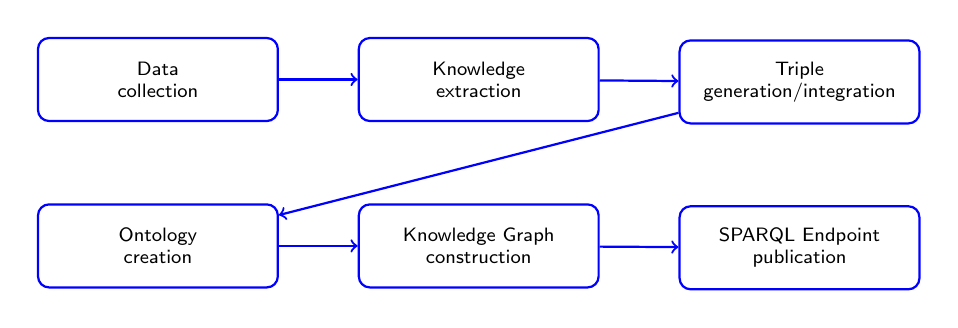
\begin{tikzpicture}[every node/.style=draw, thick, text width=8em, align=center, minimum height=3em, rounded corners, font=\scriptsize\sffamily, draw=blue]
  \matrix [matrix of nodes, column sep=1cm, row sep=1cm, draw=none, ]
  {
    |(a)| {Data\\ collection}& |(b)| {Knowledge\\ extraction}& |(c)| {Triple\\ generation/integration}\\
    |(d)| {Ontology\\ creation}& |(e)| {Knowledge Graph\\ construction}& |(f)| {SPARQL Endpoint\\ publication}\\
  };
  { [start chain,every on chain/.style={join=by ->}]
    \chainin (a);
    \chainin (b);
    \chainin (c);
    \chainin (d);
    \chainin (e);
    \chainin (f);
  }
\end{tikzpicture}
    \caption{The adopted pipeline.}
    \label{fig3}
\end{figure}

%\textbf{- KG Development:}
%A system, written in Python and implementing the pipeline described above, has been developed and is freely available in the GitHub repository\footnote{\url{https://github.com/PeppeRubini/EVA-KG}}. 
%The following sections explain how each pipeline step was handled. 
%\begin{enumerate}
%\item \textbf{Data Collection:} The reference site documents are available in English and French, but only the English versions were used. They were selected by experts in international law and are referenced in a compiled document\footnote{\url{https://github.com/PeppeRubini/EVA-KG/blob/main/data/mapping doc link.xlsx}}.\\
%A function was created to automatically download PDFs and HTML code from the website\footnote{ \url{https://hudoc.echr.coe.int/eng}} using Selenium\footnote{\url{https://selenium.dev/}}. The HTML docs provide additional case details not in the PDFs. Each sentence is then processed for knowledge extraction.
 %\item 
The successive \textbf{Knowledge Extraction} and \textbf{Triple Generation} phases focus on processing sentence files %each compiled sentence file
for extracting corresponding triples. % After collecting data, the next step involves processing it to extract triples. This process focuses on one judgment at a time, using metadata from the Case Details section of the ECHR website. 
%Currently, only the HTML files are used for this step, as they contain the necessary metadata, while triples cannot be extracted from the document body yet.
For this purpose, HTML files have been considered as more comprehensive. Processing of each sentence instantiates a \texttt{ECHRDocument} class, representing a generic ECHR document. 
%The \texttt{ECHRDocument} class was introduced to represent ECHR documents, processing only HTML files due to their inclusion of Case Detail metadata. 
The Beautiful Soup library\footnote{\url{https://beautiful-soup-4.readthedocs.io/en/latest/}} has been used to extract information, which includes converting defendant state names to Wikidata URIs and modifying the Importance Level values for consistency.
Given the $73$ selected judgments (65) and decisions (8), overall $10325$ triples have been extracted, counting $22$ distinct predicates and $5185$ distinct entities. %, 5,108 distinct subjects, and 10,325 distinct objects.
%
The extracted triples are either serialized into a JSON file or %can be 
processed via RDFLib library\footnote{\url{https://rdflib.readthedocs.io/en/stable/gettingstarted.html}}, %used to create triples. 
%The RDFLib\footnote{\url{https://rdflib.readthedocs.io/en/stable/gettingstarted.html}} library 
that facilitates the creation of triples in standard RDF format, that can then be serialized into Turtle files. A further check for redundancy elimination has been performed, but no redundancy among the triples derived from each sentence has been found. Additionally, when combining the triples from all sentences, %documents, 
RDFLib automatically removes any duplicates found across different files.

%\item \textbf{Triple Integration and Redundancy Elimination:} In this step, no specific actions were necessary because there was no redundancy among the triples derived from each sentence. Additionally, when combining the triples from all the documents, RDFLib automatically removes any duplicates found across different files.

%\item \textbf{Ontology Creation:} The ontology creation process begins by formulating competency questions\footnote{\url{https://protege.stanford.edu/publications/ontology\_development/ontology101-noy-mcguinness.html}} that the ontology-based KG is intended to address, such as: \textit{What type of document is being handled? When is the document dated? Is it possible to find the information of a specific case given its identifier? By whom is the appellant represented? To which European state does the appellant belong?} 


\begin{figure}[h]
\centering
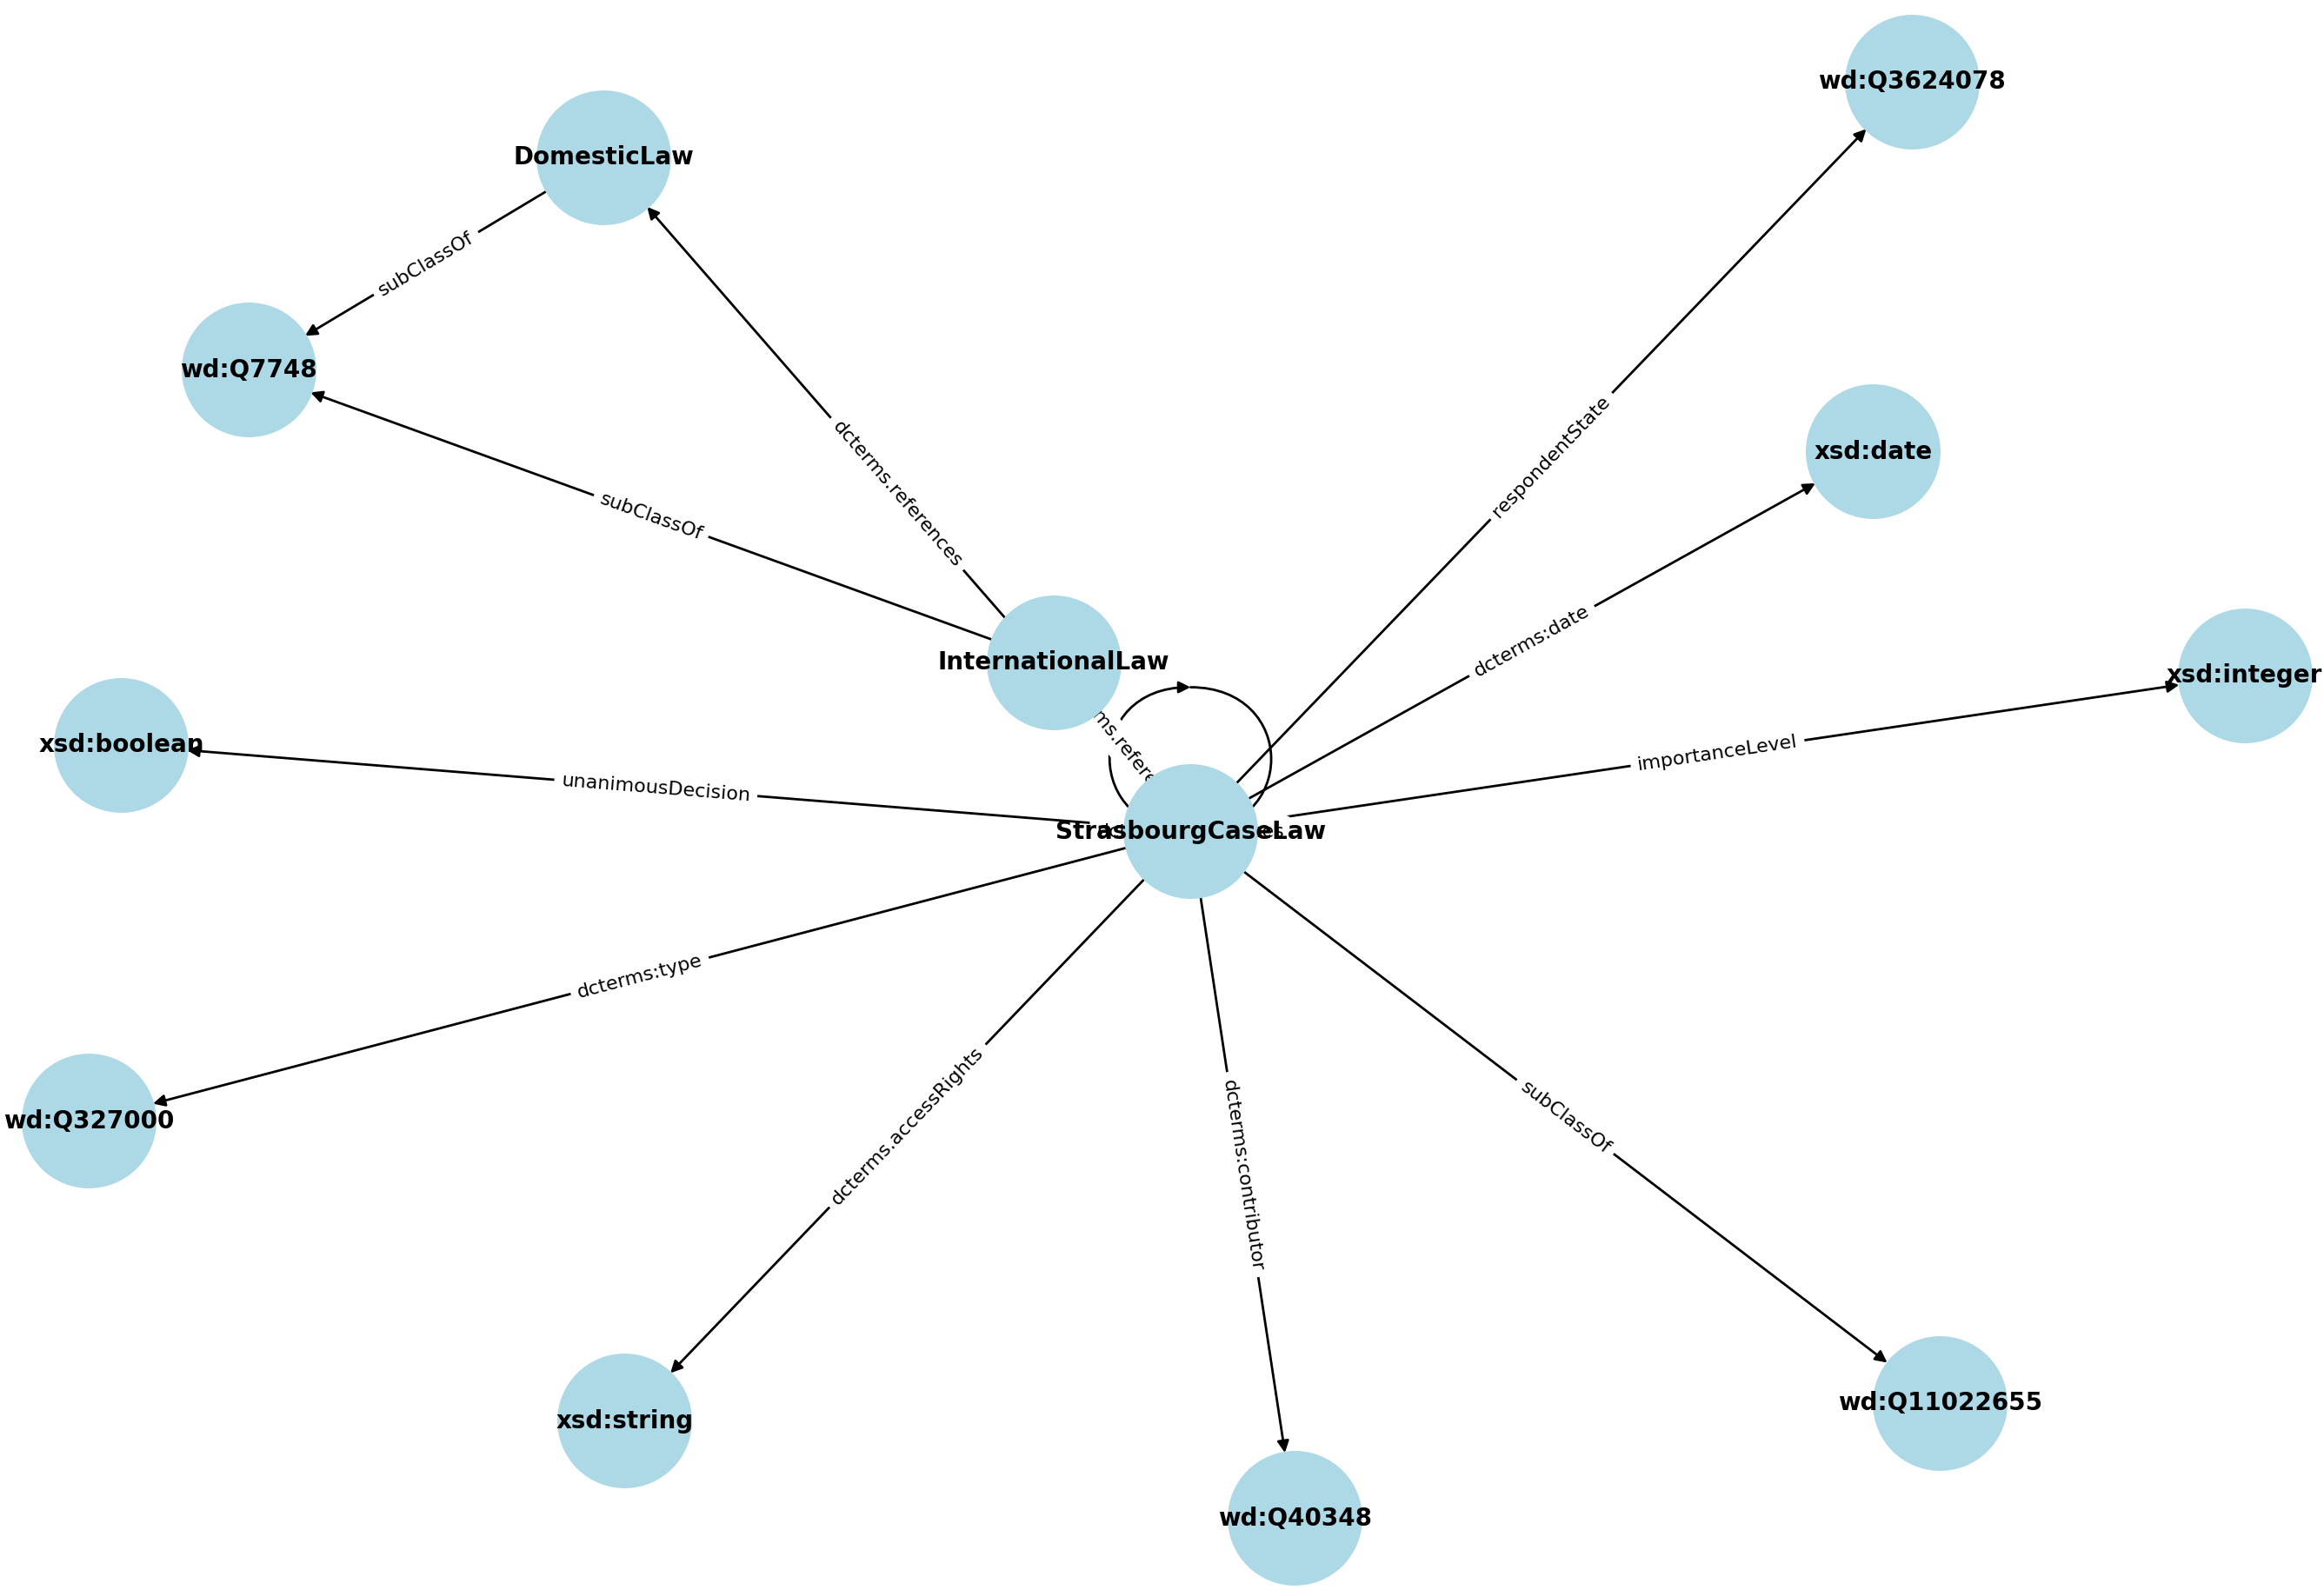
\includegraphics[width=15cm]{kg_approuach1.png}
\caption{Part of Knowledge Graph Constructed Using a Bottom-Up Approach.}
\label{KGapp1}
\end{figure}
As for the \textbf{Ontology Creation} and \textbf{KG construction}, in agreement with the ontology engineering best practices, we started with the formalization of competency questions\footnote{\url{https://protege.stanford.edu/publications/ontology\_development/ontology101-noy-mcguinness.html}} (CQs) that the ontology-based KG should address. The CQs adopted for this purpose are summarized in Tab.~\ref{tab:CQ1} (first column). %present the CQs and highlights how each of the competency questions can be answered.
For this phase, we also considered existing ontologies and vocabulary, % and metadata, 
such as ECLI, for possible reuse for %have been analyzed for their suitability in 
representing ECHR pronouncements. However, not all CQs could have been answered using the existing resources (Tab.~\ref{tab:CQ1}, second column). %data, necessitating the definition of 
Hence, new concepts/classes and properties have been defined. These new concepts include %classes like 
\texttt{DomesticLaw}, \texttt{InternationalLaw}, and \texttt{StrasbourgCaseLaw}. As for the properties, % Additional properties, such as 
\texttt{applicationNumbers}, \texttt{importanceLevel}, \texttt{respondentStates}, \texttt{involvedArticles}, and \texttt{unanimousDecisionIndicators}, have been  defined. Furthermore, new individuals, represented by URI sentences, have been created for each ruling, instantiating %and linked to 
the \texttt{StrasbourgCaseLaw} class. Figure \ref{KGapp1} illustrates a fragment of the hierarchical taxonomy of the legal concepts in the developed KG, such as \texttt{DomesticLaw} and \texttt{StrasbourgCaseLaw}, along with associated properties. All in all, the metadata %and fields 
from Case Details have been used to enrich the ECLI data and address most of the CQs. %, although some required the introduction of new data elements and structures.
%
%\item \textbf{KG Construction and visualisation:} 
The final KG has been constructed by combining the triples from various judgments and linked to external resources including %like 
Wikidata for geographic
information representation. We also developed three independent visualization solutions by adopting: % were developed: 
PyVis Library\footnote{\url{https://pypi.org/project/pyvis/}}, RDF Grapher\footnote{\url{https://www.ldf.fi/service/rdf-grapher}}, and Neo4j\footnote{\url{https://neo4j.com/}}, respectively.

%\item \textbf{Querying via SPARQL Endpoint:}
In order to query the obtained KG, we proceeded with the \textbf{SPARQL Endpoint publication}. Specifically, the SPARQL endpoint has been implemented as a Flask\footnote{\url{https://flask.palletsprojects.com/en/3.0.x/}} web application, leveraging the flexibility and simplicity of the Flask framework for web services. Flask, serves as the web
framework for handling HTTP requests, routing, and rendering responses. SPARQL 1.1 engine has been used for executing the SPARQL queries. %The key components of the implementation include: Framework and Libraries, Data Loading. 
%\textbf{Framework and Libraries:} 
%\textit{Flask}\footnote{\url{https://flask.palletsprojects.com/en/3.0.x/}} that serves as the web framework for handling HTTP requests, routing, and rendering responses. Its lightweight nature and ease of integration make it an ideal choice for developing the SPARQL endpoint. RDFLib\footnote{\url{https://rdflib.readthedocs.io/en/stable/}} a Python library that is used for working with RDF data. It supports parsing, serialization, and querying of RDF graphs, and includes a SPARQL 1.1 engine for executing SPARQL queries.\\
%\textbf{Data Loading:} 
RDF data is loaded into the RDFLib graph at application startup. The graph supports multiple serialization formats, such as Turtle, RDF/XML, and N-Triples.
The application includes two main routes: the home page (\texttt{/}) with a form for submitting queries and a query endpoint (\texttt{/query}) that processes and displays the results. The interface uses HTML templates: \texttt{INDEX.html} for query submission and \texttt{RESULT.html} for displaying results. This setup provides a user-friendly way to interact with and query RDF data.
The SPARQL endpoint, along with the full implementation of the web application, is available on the GitHub repository\footnote{\url{https://github.com/khaoulafatima/PJ4W}}.


\begin{table}[bt]%[h]
\centering
 \caption{%Table of 
 Competency Questions Adopted for the Bottom-Up Approach.}
\resizebox{\textwidth}{!}{%
\begin{tabular}{|p{10cm}|p{4cm}|} \hline 
\textbf{Question }& \textbf{Corresponding Term}\\ \hline 
What type of document are we dealing with?    & dcterms:type\\ \hline 
When is the document dated?    & dcterms:date\\ \hline 
Can I retrieve the information of a certain case given its identifier? & dcterms:isVersionOf \\ \hline 
Who represents the applicant?	& dcterms:contributor\\ \hline 
To which European state does the applicant belong?& respondentState\\ \hline 
What was the ruling?	& dcterms:abstract\\ \hline 
Was the ruling unanimous?	& unanimousDecision\\ \hline 
Which articles of the Convention were considered?& involveConventionArticle\\ \hline 
Which laws were considered to reach this conclusion?& dcterms:references\\ \hline
What is the importance of the ruling concerning future cases?&importanceLevel\\\hline
Is the document publicly accessible?	&dcterms:accessRights\\\hline
In which language is the document written?	&dcterms:language\\\hline
Where can I consult the document?	&dcterms:identifier\\\hline
    \end{tabular}
    } % resizebox
    \label{tab:CQ1}
\end{table}

%\subsubsection{Results}
%A KG focused on violence against women was created based on judgments from the European Court of Human Rights. The dataset includes 73 judgments and decisions, comprising 5,185 triples, 22 nodes, 1,747 distinct properties, 5,108 distinct subjects, and 10,325 distinct objects. It addresses competency questions related to document details, such as type, date, involved parties, and relevant laws. The KG incorporates connections to Wikidata for geographic information representation.\\
The resulting KG, publicly available%on the link; \textit{https://github.com/PeppeRubini/EVA-KG/blob/main/KG.ttl}
\footnote{\url{https://github.com/PeppeRubini/EVA-KG/blob/main/KG.ttl}}, provides a semantically rich interconnected structure that enables advanced querying and analysis of ECHR decisions pertaining to gender-based violence. It leverages established semantic web standards and vocabularies, enabling interoperability with external resources and datasets.
%
The dataset has been published as part of the LOD cloud\footnote{The {PREJUST4WOMAN} dataset can be found at: \url{https://lod-cloud.net/dataset/PREJUST4WOMAN\_PROJECT}}, adhering to the FAIR principles. %The approach source code and documentation are available on GitHub, providing access to and querying of the KG through a SPARQL endpoint. %As regards the ontology, Table \ref{tab:CQ1} presents the CQs and highlights how each of the competency questions can be answered.



\section{Legal Knowledge Graph Construction Using Large Language Models}
%\subsection{Knowledge Graph Construction Using Large Language Models}
\label{approach-LLM}
%****** What follows comes from the old basics section
Recent advances in LLM have revolutionized NLP by providing powerful tools for understanding and generating text. 
Models such as GPT-4 and Mixtral provide capabilities that extend to ontology development, KG construction, and query answering, creating new opportunities for automating knowledge engineering tasks in specialized domains. 
The LLM methodology improves accuracy and efficiency in information extraction for KG production while overcoming the constraints of existing methods \cite{chen2024information}.\\
These models can augment traditional approaches by leveraging extensive training data to infer relationships, identify patterns, and construct meaningful representations of unstructured textual data, such as court rulings and legal documents.\\
Legal document analysis technology based on LLMs, with the semantic understanding capacity and contextual modeling ability, may effectively tackle these challenges and provide powerful auxiliary tools for lawyer \cite{ammar2024prediction}. This synthesis of LLM and KG enables better understanding and generation of structured information, addressing long-standing challenges in the field.
%******* Inzio vecchio
The development of KGs for legal texts presents unique challenges due to the complexity and specificity of the domain. This approach combines the capabilities of LLMs and traditional NLP techniques to address these challenges. LLMs offer advanced capabilities for ontology generation and data extraction, while NLP techniques provide structured processing of text to ensure precision and clarity. By integrating these methods into a unified pipeline, the proposed approach leverages the strengths of both to create accurate and comprehensive KGs that are aligned with domain requirements and validated through competency questions.

Effective prompt engineering is essential for leveraging LLMs to produce desired outputs\footnote{\url{https://www.diariodiunanalista.it/posts/guida-prompt-engineering/}}. This approach utilized two key techniques: \textit{zero-shot prompting}, suitable for simple tasks with clearly expressed requirements, and \textit{few-shot prompting}, which includes examples to guide the model in handling more complex tasks and reducing errors like hallucination.\\

The proposed methodology for generating KGs from legal rulings integrates advanced LLMs and traditional NLP techniques into a cohesive workflow. It involves two pipelines, one of which is an NLP-based pipeline\footnote{\url{https://github.com/Fra3005/PreJust4Womans}}. The LLM pipeline includes document preparation, Retrieval-Augmented Generation (RAG) development, ontology and KG creation, and competency question validation, while the NLP pipeline focuses on preprocessing, POS tagging, and triple extraction for constructing KGs.
\subsubsection{KG Development}
\begin{enumerate}
\item \textbf{LLM's Pipeline}\\
\textbf{- Document Preparation:} The case study focused on analyzing and constructing KG from legal judgments, considering two distinct types of input. The first type utilized the entire judgment (full-text), while the second involved a specific sub-part of the judgment, selected by domain experts. The aim was to assess the effectiveness of both input types. For preparation, automated functions were used to extract text from PDFs for the full-text input. However, due to the varying structure and complexity of each judgment, manual extraction was employed for the sub-part input. Once the text was extracted, it was formatted into a document, ready for the subsequent steps.\\
\textbf{- RAG's Creation:} RAG models have been employed to limit the output of LLMs to the context of each specific document. Although LLMs are trained on vast amounts of data, they can sometimes struggle with providing accurate responses to specialized tasks. To address this, RAGs enhance traditional LLMs by integrating a well-defined corpus of text \cite{lewis2020retrieval}. This enables LLMs to access two types of data when responding to user queries: parametric data, which refers to the model's training data, and nonparametric data, which consists of new, external data stored in a vector container. The LLM inspects this nonparametric data to generate precise answers.\\
For the creation of RAGs, the TogetherEmbedding method \footnote{\url{https://python.langchain.com/v0.2/docs/integrations/text\_embedding/together/}} from the LangChain library was used. BERT-M2 served as the embedding model for semantic search within the vector dataset, and FAISS \footnote{\url{https://python.langchain.com/v0.1/docs/integrations/vectorstores/faiss/}}, accessed through the langchain\_community library, was used to manage the vector dataset. RAGs were created for all five documents involved, which were then used as the contextual basis for the LLM to generate responses to various prompts.
\textbf{- Base's Ontology Creations:}
At this stage, the ontology, serving as a T-box for constructing the final KGs, was developed. Initially, GPT-4.o was employed to generate a foundational ontology, as Mixtral 8x22b proved incapable of creating a general schema for this topic. Using GPT-4.o resulted in a basic ontology containing core elements such as classes (e.g.,\textit{ Abuse and LegalCase}) and \textit{ObjectProperty}. Subsequently, the ontology was enriched with additional elements using Mixtral, which, despite explicit instructions in the prompts, tended to add extra components like \textit{DataProperty }and \textit{ObjectProperty} during the KG generation process.\\
To further refine the ontology, a zero-shot prompting technique was applied to domain-specific documents. Prompts instructed the model to expand the ontology by incorporating fundamental concepts from these documents. This process was repeated with several randomly selected documents. After multiple iterations, it was observed that Mixtral consistently produced similar elements regardless of the input document. This indicated structural similarities among the documents, allowing the newly generated elements to be reused across them, effectively identifying common patterns.
Once the ontology was finalized, a thorough manual review was conducted to eliminate superfluous elements in the schema. This step addressed inconsistencies and redundancies in \textit{DataProperty} elements, ensuring the ontology aligned with the project's requirements.\\
\textbf{- KG Creation:} Building on the created ontology and the RAG for each document, a prompt engineering phase was undertaken to generate KGs for each document. This phase utilized a few-shot prompting technique to design effective prompts. Once the individual KGs were generated, they were merged into a unified graph. The merging process preserved the distinct entities from each document and ensured consistency across the combined KG.\\
\textbf{- CQ's creation and Answering:} As a final step, CQs were generated using Mixtral. For this task, the ontology was provided to the LLM with instructions to create a list of CQs based on its structure. The generated CQs aligned seamlessly with the ontology schema, eliminating the need for manual refinement. However, only a subset of the CQs was selected for further use.
Subsequently, using Mixtral, a zero-shot prompt was developed to generate answers to the selected CQs based on each document. Each answer underwent a manual verification process to ensure consistency with both the reference KG and the original text, thereby avoiding potential hallucinations. Once validated, the verified responses were formatted into a CSV file for further analysis or use.

\item \textbf{NLP's Pipeline}

\textbf{- Preprocessing:} This step, as described above, was conducted to evaluate and compare new LLM-based approaches. The process was applied to only one of the five previously analyzed documents. Initially, after the document was read and its text extracted, a preprocessing phase was carried out using the NLTK library \footnote{\url{https://www.nltk.org/}}. This phase involved several steps, including punctuation removal, tokenization, stopword removal, and lemmatization, to prepare the text for subsequent analysis.\\
\textbf{- Part of Speech:} After tokenization, the SpaCy library was used to perform POS tagging for each token. POS tagging is a NLP technique that categorizes the components of a sentence, making it particularly valuable for complex tasks like Sentiment Analysis or Machine Translation. In this study, POS tagging was utilized to extract triples from the document. Tokens were categorized into "subj" (subject), "verb," and "obj" (object) based on their grammatical roles, enabling the creation of structured triples.\\
\textbf{- Triples Creation:} In the final step of the pipeline, triples were constructed by associating each identified subject with its corresponding verb and object. This process resulted in a structured representation of the text, capturing meaningful relationships between entities within the document.

\end{enumerate}
\begin{table}[t]
\centering
\caption{Score CQs answering of Large Language Models Approach.}\label{tab1}
\resizebox{0.7\textwidth}{!}{
\begin{tabular}{|l|c|c|}
\hline
\textbf{Results} &  \textbf{Full-text} & \textbf{Sub-part}\\
\hline
Which legal case is associated with Violation? & 3 & 4\\
\hline
What is the legal outcome of Case? & 4& 4\\
\hline
What is the reason stated for the judgment? &4 & 2\\
\hline
What abuse is related to Judgment? &  5& 4\\
\hline
What is the severity level of Abuse? &2 & 2\\
\hline
What is the duration and frequency of Abuse? &3& 2\\
\hline
Which legal articles are violated? & 4& 4\\
\hline
What is the context of Abuse?& 5& 4\\
\hline
Which court judged the Case? & 2& 1\\
\hline
What are the damages related to Judgment? &1& 3\\
\hline
What are the consequences of Abuse? &5&4\\
\hline
How much in legal damages and costs were awarded? & 0& 4\\
\hline
What is the legal status? & 5& 3\\
\hline
\multicolumn{1}{|r|}{\textbf{Total}} & \textbf{40/65}& \textbf{37/65}\\
\hline
\end{tabular}
}
\end{table}

\subsubsection{Empirical Evaluation}
To evaluate the LLM-based KG generation pipeline, we relied on a qualitative analysis based on answers to CQs. As detailed in Table 2, each of the five documents was associated with 13 CQs. These were answered by the LLM-generated KGs and manually verified against the source text. The full-text strategy yielded 40 consistent answers out of 65 (61.5\%), while the sub-part strategy provided 37 valid answers (56.9\%). This highlights a trade-off: full-text inputs offer broader coverage, while sub-part inputs although narrower yield more focused and relevant results, especially for factual or procedural queries. This CQ-based evaluation provided a useful lens into the structure, coverage, and correctness of the generated knowledge.



\subsubsection{Results}
This approach examines the role of LLMs in knowledge engineering tasks, including ontology generation, instance creation, and evaluation against traditional NLP methods. In generating ontologies, the LLM struggled to independently create a complete domain-specific ontology using only its pretrained knowledge, requiring additional domain-specific documents for specialization and highlighting the need for expert oversight in nuanced domains. Although the ontology generally performed well, the LLM occasionally failed to generate complete or accurate instances, even when tailored to the document structure, emphasizing the necessity of human validation to ensure correctness.


\begin{figure}[h]
\centering
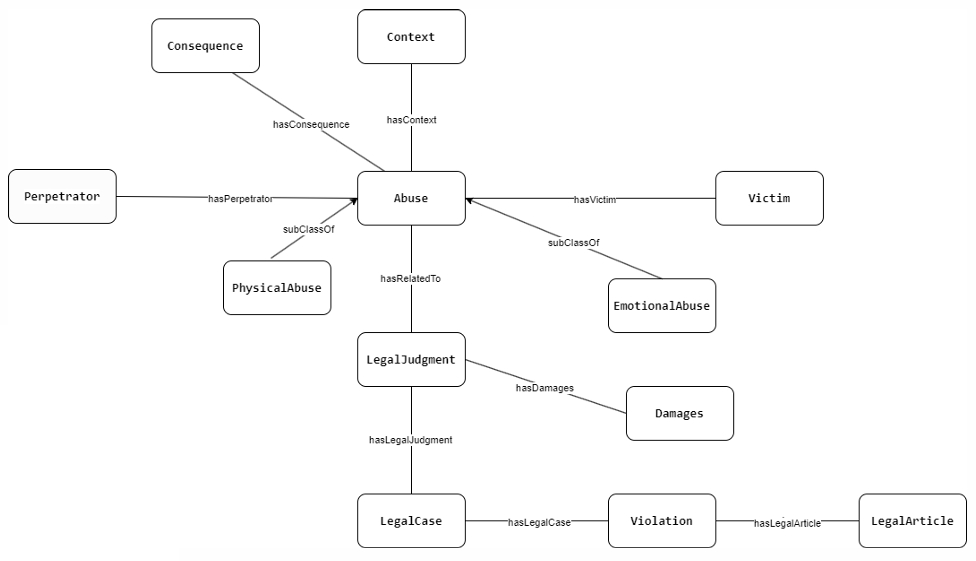
\includegraphics[width=10cm]{llm_approach_kg.png}
\caption{Part of Knowledge Graph Constructed Using Large Language Models.}
\label{KGLLM}
\end{figure}

Two specific use cases were explored to evaluate the effectiveness of LLMs in document processing:\\
\textbf{\textit{Full-text approach:}} This use case involved processing the entire document to construct KGs and answer Competency Questions. While this approach provided the highest quantity of responses due to its comprehensive coverage, the relevance and accuracy of the responses varied. Full-text processing captured more nuanced information but required significant manual verification to filter out irrelevant or incorrect outputs. The technical challenges included longer processing times and token size limitations inherent in LLMs.\\
\textbf{\textit{Sub-part approach:}} This approach utilized text segments selected by domain experts, focusing on parts deemed most relevant to the analysis. Although this method produced fewer responses compared to the full text approach, it offered a higher likelihood of alignment with the objectives of the experts. It was faster, avoided token limitations, and facilitated targeted processing. However, it required precise expert input to ensure that no critical information was excluded.\\
The evaluation of the CQs, detailed in Table\ref{tab1}, focused on responses consistent with the text, excluding incomplete entities generated by the LLM only to establish links. The resulting KG, as defined in the GitHub repository \footnote{https://github.com/Fra3005/PreJust4Womans/blob/main/Commons/final\_onto.ttl},  represents structured knowledge derived from domain-specific legal and policy documents addressing women's rights and gender-based issues. It encapsulates core concepts, along with their semantic relationships comprising 12 classes, 9 object properties, 17 data properties, capturing the conceptual structure of the domain without populated example instances, as depicted in figure\ref{KGLLM}. This KG driven structure supports the instantiation of real-world scenarios discussed in source documents and serves as a foundation for answering CQs.\\
The CQs were classified according to relevance in the context of the study and their accuracy was confirmed by manual verification against the source documents. The comparison of these two use cases highlighted that while the full-text approach excels in information quantity, the sub-part approach proves more effective for specific, domain-oriented tasks. These findings underscore the importance of balancing comprehensive data processing with precision, guided by expert judgment, to maximize the utility and accuracy of LLM outputs.


\section{Discussion} \label{disc}

\subsection{Comparative Overview: Bottom-Up vs LLM-Based Approaches}
In this work we have proposed two distinct methodologies for constructing KGs to address legislation on violence against women: a bottom-up approach and an LLM-based approach. %Each method was developed to optimize the generation of KGs for predictive justice tasks, with unique strengths and limitations. 
This section discusses the two approaches, comparing their methodologies, outputs, and suitability for our purpose. A summary of the discussion is provided in 
Tab.~\ref{tab:tab2}.  



\begin{table}[h]
\centering
\caption{Comparative Analysis of Bottom-Up and LLM-Based Approaches.}
\resizebox{1\textwidth}{!}{%
\begin{tabular}{|p{3.5cm}|p{8cm}|p{8cm}|}\hline
\textbf{Criteria} &  \textbf{Bottom-Up Approach} & \textbf{LLM-Based Approach} \\ \hline
Methodology & Structured pipeline & Combine LLM capabilities with NLP and RAG techniques \\ \hline
Strengths& High precision and semantic alignment; Reliable for domain-specific; Structured tasks & Fast and scalable KG creation\\ \hline
Challenges& Labor-intensive and time consuming; less adaptable to novel or unexpected patterns  & Accuracy issues (hallucination and token limits \\ \hline
Performance on CQs &Excels in precise, structured queries using semantic standards  & Generate broader responses but needs post-processing to ensure relevance\\ \hline
Use Case Suitability & Best for formal legal reasoning and SPARQL-based tasks & Ideal for exploratory tasks, large scale processing, and rapid prototyping\\ \hline
Scalability & Limited scalability due to manual data processing & Highly scalable for diverse and large datasets \\ \hline
Output Consistency  & Outputs are precise and domain-aligned  & Outputs may vary in consistency and require refinement \\ \hline
Ontology Adaptability & Limited to predefined ontologies & Highly adaptable to diverse and nuanced data patterns \\ \hline
Ontology Concepts & Higher initially, with many specific concepts emerging from data & More limited, well-organized in a clear hierarchy \\ \hline
Ontology Relations & More dynamic, based on frequently occurring relations in data & Accurate and based on logical modeling \\ \hline
Ontology Size & Large in size (583.7 KB), including a more extensive set of classes, properties, and relationships  & Smaller in size (6.4 KB), suggesting a more concise ontology with potentially fewer classes and relationships \\ \hline
\end{tabular}
} 
\label{tab:tab2}
\end{table}



The bottom-up approach %, grounded in traditional knowledge engineering principles, 
follows a systematic pipeline (involving data collection, knowledge extraction, triple integration, and ontology creation), ensuring the development of %robust, 
%semantically aligned 
a KG, tailored for ECHR judgments, that is aligned and interlinked to existing resources, e.g. ECLI and Wikidata. %It excels 
This methodology resulted appropriate for delivering rather precise, domain-specific output, making it ideal for tasks requiring strict adherence to the available sources of knowledge and to existing semantically related resources. However, it is resource intensive, time-consuming, and less adaptable %to novel data patterns 
due to its reliance on predefined ontologies. In contrast, the LLM-based approach resulted a bit less structured in its process but rather flexible, leveraging advanced natural language processing and prompting techniques, such as zero-shot and few-shot prompting and retrieval-augmented generation, to accelerate ontology and KG creation. This approach is more scalable (given trained LLMs), adaptable to various legal texts, and capable of capturing nuanced information from full-text and expert selection document parts. Nevertheless, it faces challenges in accuracy and consistency, requiring extensive manual validation to avoid issues like hallucination and incomplete entities. While the bottom-up approach is suited for applications requiring precision, consistency, and semantic accuracy, such as formal legal reasoning and SPARQL-based querying, the LLM-based approach is more suitable for exploratory tasks, rapid prototyping, and large-scale data processing, where speed and adaptability are prioritized over perfect accuracy. 

%By blending FAIR principles with the reuse of existing ontologies, our KG provides a robust foundation for tackling domain-specific challenges. The methodologies applied—bottom-up extraction and Large Language Model-assisted creation—not only enhanced the KG's semantic richness but also promoted its alignment with global legal standards. This strategic integration ensures that the resource is both innovative and practical, serving as a reliable component in legal AI applications.

\subsection{Ontology Development}
The project resulted in two ontologies; one generated using a Large Language Model, and one through a bottom-up approach. The automatic generated ontology, while efficient and scalable, was minimal and included generic classes due to the absence of domain specific constraints. In contrast, The manually constructed ontology was more semantically rich and aligned with legal reasoning needs. It introduced targeted classes to address specific gaps and accurately reflect legal structures. This comparison underscores the complementary value of both approaches and highlights the necessity of expert refinement when high legal fidelity is required. 

The demonstrated feasibility of combining structured extraction and LLM-based techniques opens new possibilities for semi-automated legal knowledge engineering pipelines. This hybrid approach could inform and the design of scalable KG generation frameworks across other legal domains, thereby contributing to the democratization of legal data access and interpretability in predictive justice systems. These findings underscore the importance of balancing comprehensive data processing with precision, guided by expert judgment, to maximize the utility and accuracy of LLM outputs. 

\subsection{Ensuring FAIRness in Legal Knowledge Engineering}
The developed Legal Knowledge Graph adheres to the FAIR (Findable, Accessible, Interoperable, and Reusable) principles through the following mechanisms:
\begin{itemize}
\item \textbf{Findable:} The KG is assigned a persistent DOI (https://doi.org/10.5281/zenodo.15270173) and is registered in the LOD Cloud (https://lod-cloud.net/dataset/PREJUST4WOMAN\_PROJECT), ensuring long-term retrievability and discoverability.
\item \textbf{Accessible:} The resource is openly accessible via Zenodo and GitHub, with no access restrictions. The KG is also exposed through a public SPARQL endpoint enabling both human and machine access.
\item \textbf{Interoperable:} The KG is published in standard RDF/Turtle format and relies on widely adopted vocabularies and ontologies, allowing integration with other legal and governmental data.
\item \textbf{Reusable:} The dataset is released under a permissive Creative Commons Attribution 4.0 International License, with complete documentation and source code available via GitHub. This enables others to reuse, extend, and adapt the resource for legal AI applications or broader knowledge engineering tasks.
\end{itemize}

\subsection{Quantitative Evaluation of Precision and Quality}
The evaluation provides a clearer understanding of the differences and complementarities between the two methodologies. The bottom-up approach emphasizes semantic precision, relying on structured extraction pipelines, curated ontologies, and expert-defined competency questions. This results in well-aligned, interpretable outputs that are suitable for formal legal reasoning and SPARQL querying. On the other hand, the LLM-based approach offers higher adaptability and faster development by leveraging retrieval-augmented generation and prompt engineering. While the automatically generated outputs require human oversight to ensure relevance and avoid hallucinations, they demonstrate strong potential for rapid KG bootstrapping and domain exploration. Competency questions were employed in both approaches: in the bottom-up pipeline, they guided ontology design and validation; in the LLM pipeline, they served as a mechanism to test the informativeness of generated graphs. Overall, the two approaches are complementary—manual engineering ensures domain fidelity and interpretability, while LLM-based methods enable scalability and prototyping across diverse legal texts.


\section{Conclusion}\label{conc}
With this paper, we %This study has 
introduced a novel %and comprehensive 
Legal Knowledge Graph focused on legislation addressing violence against women. %The developed KGs significantly enhances legal reasoning by enabling detailed analyses of judicial decisions, improving query answering for legal professionals, and supporting predictive justice applications. 
Designed in accordance with FAIR principles, the Legal KG ensures interoperability and possibly reusability across legal and AI systems. %, ultimately promoting transparency and efficiency in legal processes. These contributions represent a vital step toward intelligent, data-driven legal systems capable of addressing complex gender-based legal issues.\\
To construct the KG, two automated methodologies have been adopted/tailored: a %structured 
bottom-up approach and an %adaptive 
LLM-based approach. Each methodology offers distinct advantages: precision and domain-specific accuracy for the case of the bottom-up solution; scalability and flexibility for case of the LLM-based approach. %Together, they support key legal tasks such as detailed judicial analysis, enhanced query answering, and predictive justice integration.\\

Future work will focus on merging the two KGs into a unified resource, to be possibly expanded and on extending the KG applicability %to specific tasks, including 
to the automated detection of legal patterns. %, improved access to case information, and support for targeted policy-making. This will involve enriching the KG with additional triples from both structured and unstructured legal texts, refining ontologies with expert input, and merging the two KGs into a unified resource. 
%Further developments will also include integrating advanced NLP and LLM techniques, building task-specific tools and predictive models, and extending 
Additionally, we are planning to experimenting the applicability of the proposed methodologies %the approach 
to other legal domains in order to showcase the generality of the proposed solutions and ultimately contributing to a unified, FAIR-aligned representation of European laws that may enhance % that enhances 
legal automation and judicial efficiency.
     

\begin{credits}
    \subsubsection{\ackname}
    This work was partially supported by project \emph{FAIR - Future AI Research} (PE00000013), spoke 6 - Symbiotic AI (\url{https://future-ai-research.it/}) under the PNRR MUR program funded by the European Union - NextGenerationEU, and by PRIN project \emph{HypeKG - Hybrid Prediction and Explanation with Knowledge Graphs} (Prot. 2022Y34XNM, CUP H53D23003700006) under the PNRR MUR program funded by the European Union - NextGenerationEU
\end{credits}
%
% ---- Bibliography ----
%
% BibTeX users should specify bibliography style 'splncs04'.
% References will then be sorted and formatted in the correct style.
%

\bibliographystyle{splncs04}
\bibliography{biblio}

\end{document}
